\documentclass{beamer}

\usepackage{framed}
\usepackage{graphicx}

\begin{document}
	
\section{Sequential color palettes}
%====================================%
\begin{frame}[fragile]
\frametitle{Seaborn Workshop}
\large

\textbf{Sequential color palettes}
\begin{itemize}
\item The second major class of color palettes is called “sequential”. This kind of color mapping is appropriate when data range from relatively low or unintersting values to relatively high or interesting values. 
\item Although there are cases where you will want discrete colors in a sequential palette, it’s more common to use them as a colormap in functions like \texttt{kdeplot()} or \texttt{corrplot()} (along with similar matplotlib functions).
\end{itemize}

\end{frame}
%====================================%
\begin{frame}[fragile]
	
	\frametitle{Seaborn Workshop}
	\large
\begin{itemize}
\item It’s common to see colormaps like jet (or other rainbow palettes) used in this case, becuase the range of hues gives the impression of providing additional information about the data. 
\item However, colormaps with large hue shifts tend to introduce discontinuities that don’t exist in the data, and our visual system isn’t able to naturally map the rainbow to quantitative distinctions like “high” or “low”. 
\item The result is that these visualizations end up being more like a puzzle, and they obscure patterns in the data rather than revealing them. 
\item The jet palette is particularly bad because the brightest colors, yellow and cyan, are used for intermediate data values. This has the effect of emphasizing uninteresting (and arbitrary) values while demphasizing the extremes.
\end{itemize}
\end{frame}
%====================================%
\begin{frame}[fragile]
	\frametitle{Seaborn Workshop}
	\large
For sequential data, it’s better to use palettes that have at most a relatively subtle shift in hue accompanied by a large shift in brightness and saturation. This approach will naturally draw the eye to the relatively important parts of the data.
\end{frame}
%====================================%
\begin{frame}[fragile]
\frametitle{Seaborn Workshop}
\large

The Color Brewer library has a great set of these palettes. They’re named after the dominant color (or colors) in the palette.
\begin{verbatim}
sns.palplot(sns.color_palette("Blues"))
\end{verbatim}

\begin{figure}
	\centering
	
\includegraphics[width=0.7\linewidth]{images/color_palettes_25_0}
\end{figure}
\end{frame}
%====================================%
\begin{frame}[fragile]
	\frametitle{Seaborn Workshop}
	\large
	Like in matplotlib, if you want the lightness ramp to be reversed, you can add a \texttt{\_r} suffix to the palette name.
\begin{verbatim}
sns.palplot(sns.color_palette("BuGn_r"))
\end{verbatim}

\begin{figure}
	\centering
	
\includegraphics[width=0.7\linewidth]{images/color_palettes_27_0}
\end{figure}


\end{frame}
%====================================%
\begin{frame}[fragile]
	\frametitle{Seaborn Workshop}
	\large
\begin{itemize}
\item Seaborn also adds a trick that allows you to create “dark” palettes, which do not have as wide a dynamic range. 
\item This can be useful if you want to map lines or points sequentially, as brighter-colored lines might otherwise be hard to distinguish.
\end{itemize}

\end{frame}
%====================================%
\begin{frame}[fragile]
	\frametitle{Seaborn Workshop}
	\large
	
\begin{verbatim}
sns.palplot(sns.color_palette("GnBu_d"))
\end{verbatim}

\begin{figure}
	\centering
	
\includegraphics[width=0.7\linewidth]{images/color_palettes_29_0}
\end{figure}
\end{frame}
%====================================%
\begin{frame}[fragile]
	\frametitle{Seaborn Workshop}
	\large
	\begin{itemize}
\item Remember that you may want to use the \texttt{choose\_colorbrewer\_palette()} function to play with the various options, and you can set the \texttt{as\_cmap} argument to \texttt{True} if you want the return value to be a colormap object that you can pass to seaborn or matplotlib functions.
	\end{itemize}

\end{frame}
\section{Sequential palettes with \texttt{cubehelix\_palette()}}
%====================================%
\begin{frame}[fragile]
	\frametitle{Seaborn Workshop}
	\large
\noindent \textbf{Sequential palettes with \texttt{cubehelix\_palette()}}
\begin{itemize}
\item The cubehelix color palette system makes sequential palettes with a linear increase or decrease in brightness and some variation in hue. 
\item This means that the information in your colormap will be preserved when converted to black and white (for printing) or when viewed by a colorblind individual.
\end{itemize}

\end{frame}
%====================================%
\begin{frame}[fragile]
\frametitle{Seaborn Workshop}
\large

Matplotlib has the default cubehelix version built into it:
\begin{verbatim}
sns.palplot(sns.color_palette("cubehelix", 8))
\end{verbatim}

\begin{figure}
	\centering
	
\includegraphics[width=0.7\linewidth]{images/color_palettes_32_0}
\end{figure}
Seaborn adds an interface to the cubehelix system so that you can make a variety of palettes that all have a well-behaved linear brightness ramp.
\end{frame}
%====================================%
\begin{frame}[fragile]
	\frametitle{Seaborn Workshop}
	\large
The default palette returned by the seaborn \texttt{cubehelix\_palette()} function is a bit different from the matplotlib default in that it does not rotate as far around the hue wheel or cover as wide a range of intensities. It also reverses the order so that more important values are darker:
\end{frame}
%====================================%
\begin{frame}[fragile]
	\frametitle{Seaborn Workshop}
	\large
	\begin{verbatim}
sns.palplot(sns.cubehelix_palette(8))
	\end{verbatim}

\begin{figure}
\centering

\includegraphics[width=0.7\linewidth]{images/color_palettes_34_0}
\end{figure}

\end{frame}
%====================================%
\begin{frame}[fragile]
\frametitle{Seaborn Workshop}
\large

Other arguments to cubehelix\_palette() control how the palette looks. The two main things you’ll change are the start (a value between 0 and 3) and rot, or number of rotations (an arbitrary value, but probably within -1 and 1),
\begin{verbatim}
sns.palplot(sns.cubehelix_palette(8, start=.5, rot=-.75))
\end{verbatim}

\begin{figure}
	\centering
	
\includegraphics[width=0.7\linewidth]{images/color_palettes_36_0}
\end{figure}

You can also control how dark and light the endpoints are and even reverse the ramp:
\end{frame}
%====================================%
\begin{frame}[fragile]
	\frametitle{Seaborn Workshop}
	\large
	By default you
\begin{verbatim}
sns.palplot(sns.cubehelix_palette(8, start=2, rot=0, dark=0, light=.95, reverse=True))
\end{verbatim}

\begin{figure}
	\centering
	
\includegraphics[width=0.7\linewidth]{images/color_palettes_38_0}
\end{figure}


\end{frame}
%====================================%
\begin{frame}[fragile]
	\frametitle{Seaborn Workshop}
	\large
By default you just get a list of colors, like any other seaborn palette, but you can also return the palette as a colormap object that can be passed to seaborn or matplotlib functions using as_cmap=True.

\end{frame}
%====================================%
\begin{frame}[fragile]
	\frametitle{Seaborn Workshop}
	\large
	
	\begin{verbatim}
x, y = np.random.multivariate_normal([0, 0], [[1, -.5], [-.5, 1]], size=300).T
cmap = sns.cubehelix_palette(light=1, as_cmap=True)
sns.kdeplot(x, y, cmap=cmap, shade=True);
\end{verbatim}
\begin{figure}
\centering
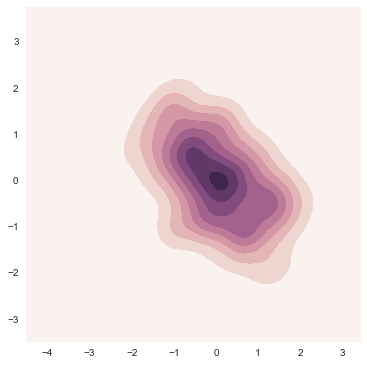
\includegraphics[width=0.7\linewidth]{images/color_palettes_40_0}
\caption{}
\label{fig:color_palettes_40_0}
\end{figure}

\end{frame}
%====================================%
\begin{frame}[fragile]
\frametitle{Seaborn Workshop}
\large
\begin{itemize}
\item To help select good palettes or colormaps using this system, you can use the \texttt{choose\_cubehelix\_palette()} function in a notebook to launch an interactive app that will let you play with the different parameters. 
\item Pass \texttt{as\_cmap=True} if you want the function to return a colormap (rather than a list) for use in function like hexbin.
\end{itemize}

\end{frame}
\section{Custom sequential palettes with \texttt{light\_palette()} and \texttt{dark\_palette()}}
%====================================%
\begin{frame}[fragile]
	\frametitle{Seaborn Workshop}
	\large
\begin{itemize}
\item For a simpler interface to custom sequential palettes, you can use \texttt{light\_palette()} or \texttt{dark\_palette()}, which are both seeded with a single color and produce a palette that ramps either from light or dark desaturated values to that color. 
\item These functions are also accompanied by the \texttt{choose\_light\_palette()} and \texttt{choose\_dark\_palette()} functions that launch interactive widgets to create these palettes.
\end{itemize}

\end{frame}
%====================================%
\begin{frame}[fragile]
	\frametitle{Seaborn Workshop}
	\large
	\begin{verbatim}
sns.palplot(sns.light_palette("green"))
	\end{verbatim}

\begin{figure}
\centering

\includegraphics[width=0.7\linewidth]{images/color_palettes_43_0}
\caption{}
\label{fig:color_palettes_43_0}
\end{figure}

\end{frame}
%====================================%
\begin{frame}[fragile]
	\frametitle{Seaborn Workshop}
	\large
\begin{verbatim}
sns.palplot(sns.dark_palette("purple"))
\end{verbatim}	


\begin{figure}
\centering

\includegraphics[width=0.7\linewidth]{images/color_palettes_44_0}
\caption{}
\label{fig:color_palettes_44_0}
\end{figure}

\end{frame}
%====================================%
\begin{frame}[fragile]
	\frametitle{Seaborn Workshop}
	\large
These palettes can also be reversed.
\begin{verbatim}
sns.palplot(sns.light_palette("navy", reverse=True))
\end{verbatim}
\begin{figure}
\centering

\includegraphics[width=0.7\linewidth]{images/color_palettes_46_0}
\caption{}
\label{fig:color_palettes_46_0}
\end{figure}


\end{frame}
%====================================%
\begin{frame}[fragile]
\frametitle{Seaborn Workshop}
\large

They can also be used to create colormap objects rather than lists of colors.
\begin{verbatim}
pal = sns.dark_palette("palegreen", as_cmap=True)
sns.kdeplot(x, y, cmap=pal);
\end{verbatim}

\begin{figure}
\centering
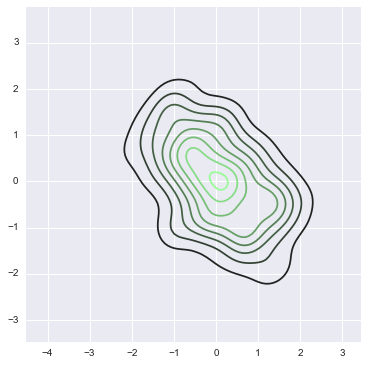
\includegraphics[width=0.7\linewidth]{images/color_palettes_48_0}
\caption{}
\label{fig:color_palettes_48_0}
\end{figure}

By default, the input can be any valid matplotlib color. Alternate interpretations are controlled by the input argument. Currently you can provide tuples in hls or husl space along with the default rgb, and you can also seed the palette with any valid xkcd color.
\end{frame}
%====================================%
\begin{frame}[fragile]
	\frametitle{Seaborn Workshop}
	\large
	\begin{verbatim}
sns.palplot(sns.light_palette((210, 90, 60), input="husl"))
\end{verbatim}
\begin{figure}
\centering

\includegraphics[width=0.7\linewidth]{images/color_palettes_50_0}
\caption{}
\label{fig:color_palettes_50_0}
\end{figure}

\end{frame}
%====================================%
\begin{frame}[fragile]
	\frametitle{Seaborn Workshop}
	\large
\begin{verbatim}
sns.palplot(sns.dark_palette("muted purple", input="xkcd"))
\end{verbatim}
\begin{figure}
	\centering
	
\includegraphics[width=0.7\linewidth]{images/color_palettes_51_0}
\end{figure}

Note that the default input space for the interactive palette widgets is husl, which is different from the default for the function itself, but much more useful in this context.
\end{frame}

\end{document}
